\subsection{La classe Object et ses fils}

Pour rappel, la classe object permet de définir toutes les entités du jeu.
Tout type définit par l'utilisateur hérite de cette classe ou de l'une de ces classes filles.
Elles sont présentées dans le schéma ci-dessous :

\begin{figure}[h]
 \centering
 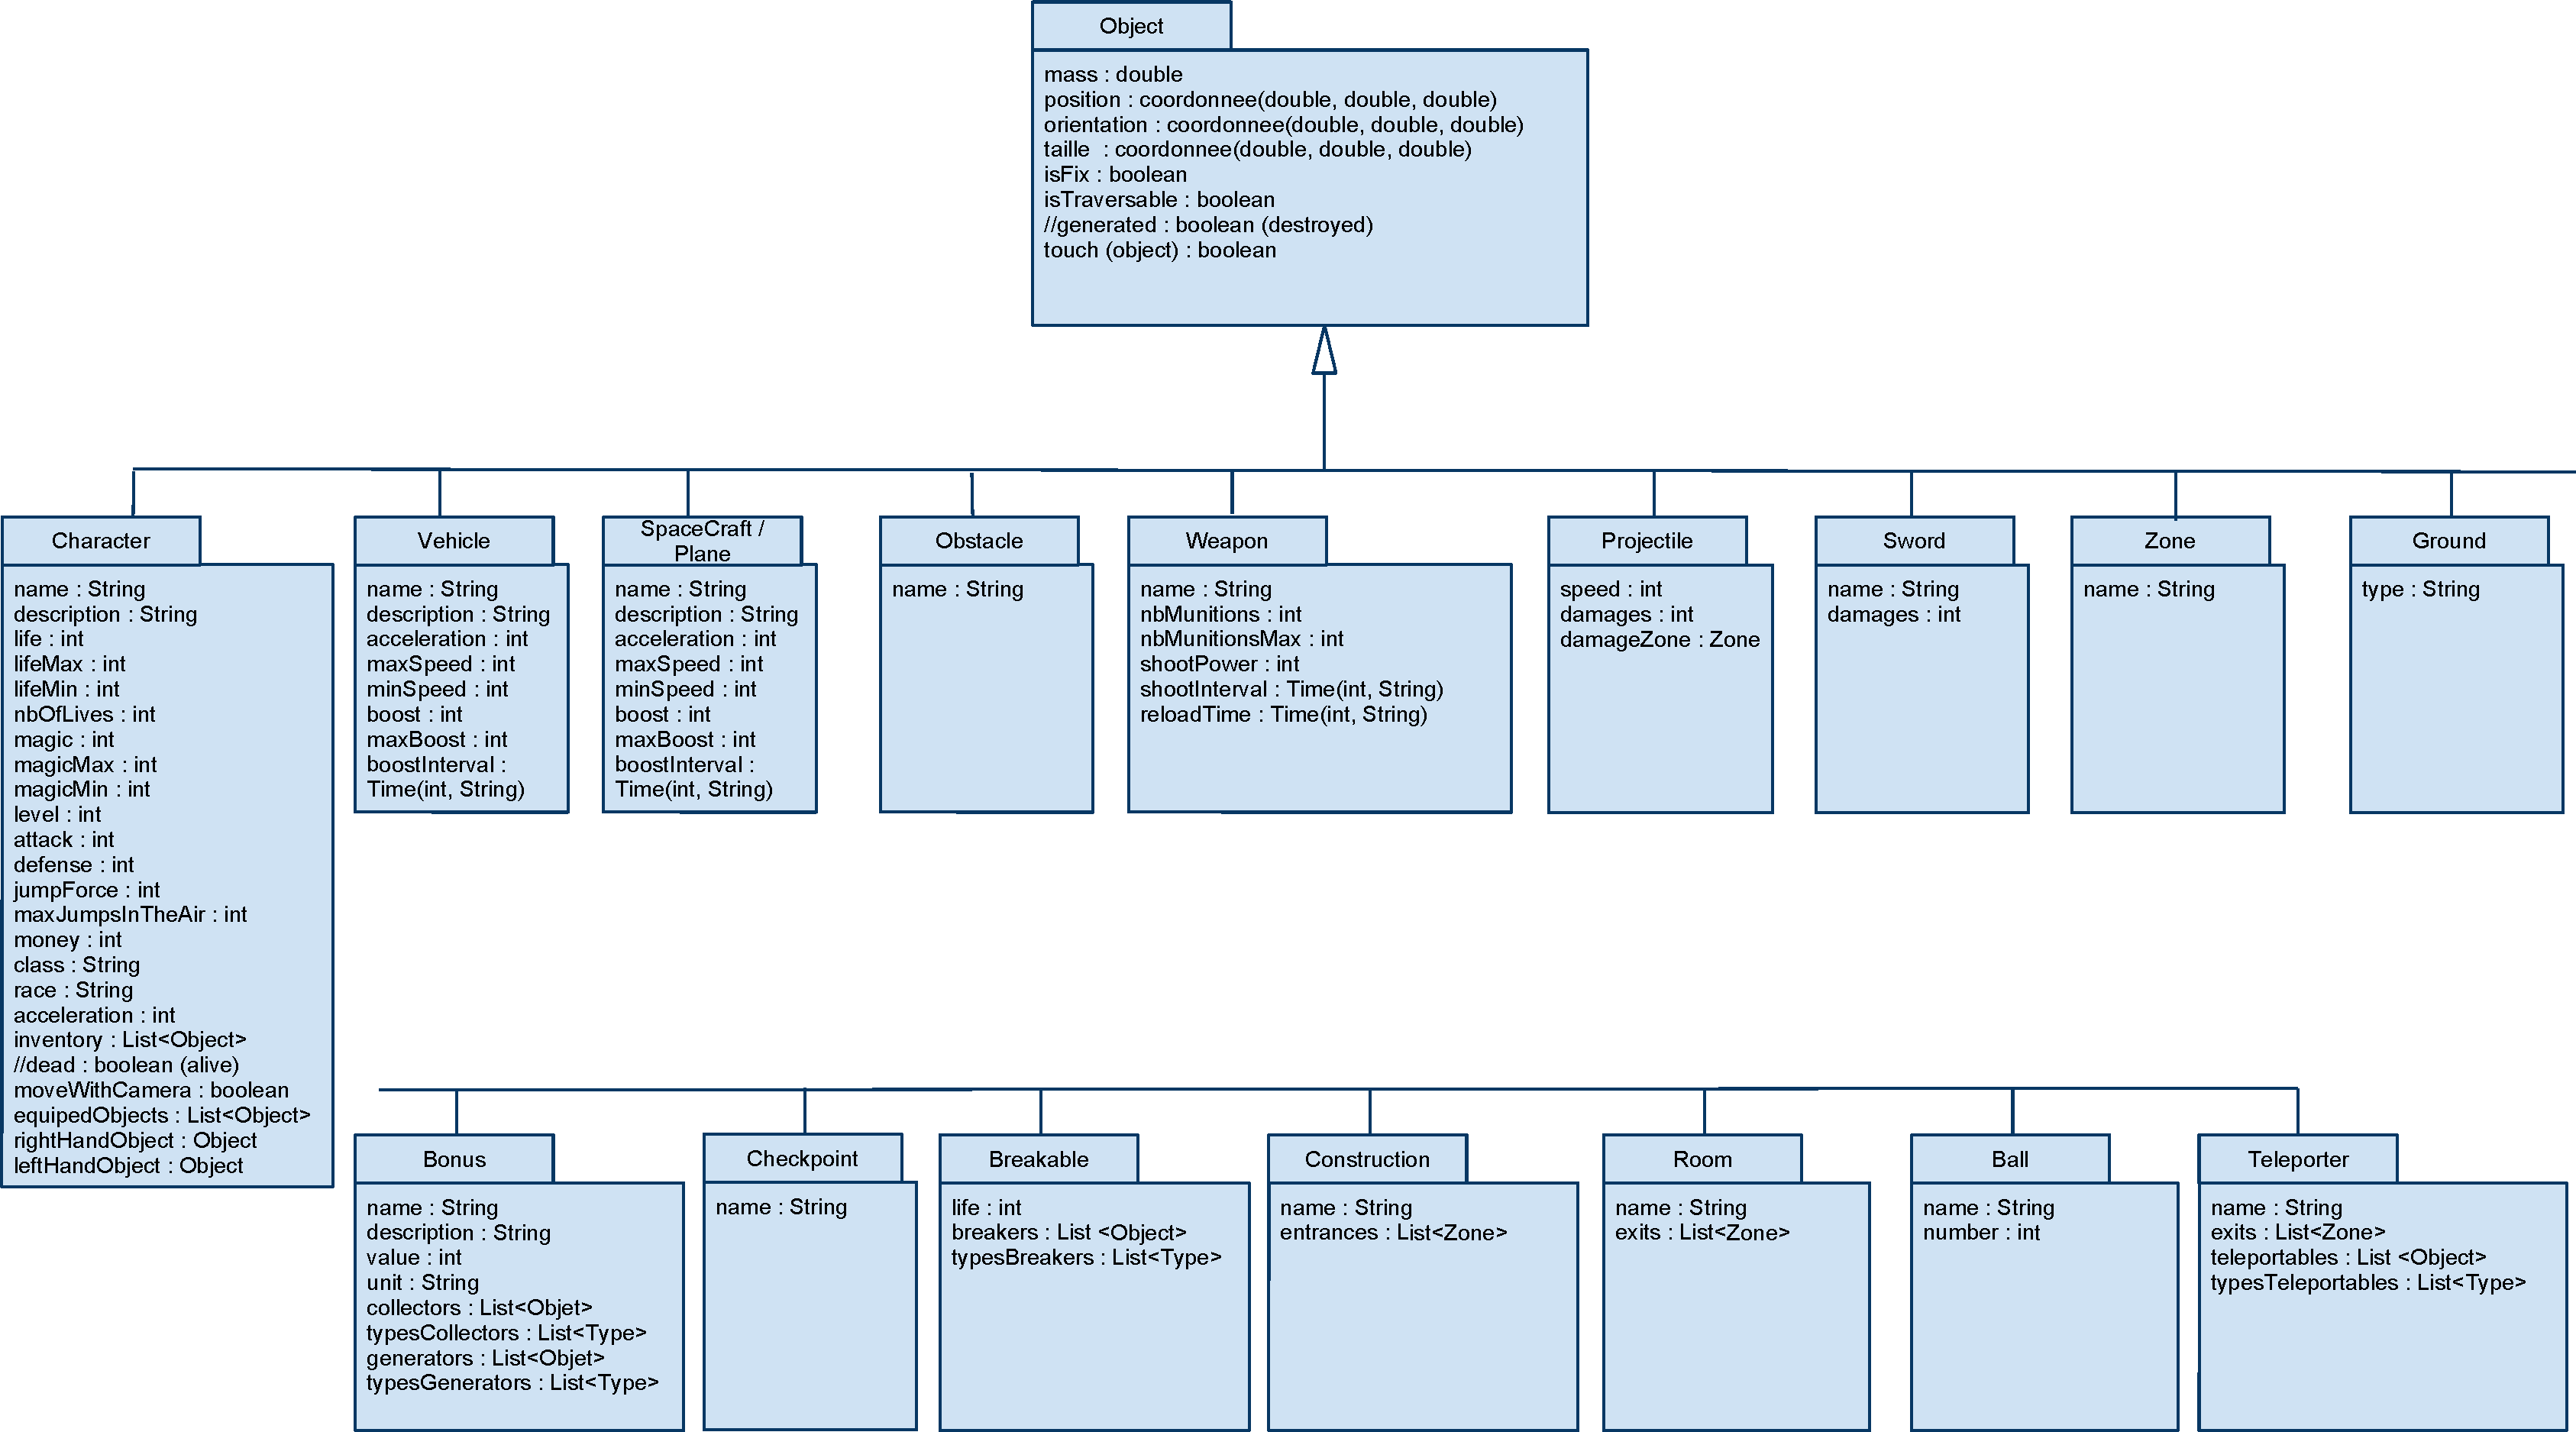
\includegraphics[width=\textwidth]{img/objectclass}
\end{figure}

Les divers attributs name pourront servir lors de l'affichage d'information.
\code{gandalf is Character. gandalf has name at 'Gandalf le Blanc'.}

Pour la classe Character, si l'accélération est bien défini, c'est elle qui régit le déplacement et les touches pour se déplacer la modifie.
Sinon le déplacement se fait directement lors de l'appui des touches.

Les classes Character, Vehicle et Plane ont des comportements différents concernant la caméra.
Par exemple, pour un déplacement vers la droite, le personnage va à droite sur l'écran, le véhicule tourne à droite, l'avion fait une rotation dans le sens horaire.

Pour les obstacles, ils héritent des attributs isFix et isTraversable de Object qui sont mis respectivement à true et false.

Concernant les projectiles, ils se déplacent jusqu'à leur description ont ils font des dégâts.

Une zone correspond juste à un volume englobant invisible, et est donc traversable par tous.

La classe Ground peut avoir plusieurs types comme la neige, qui a donc un coefficient de frottement faible, ou l'eau qui est traversable.

Un bonus possède une liste d'objets qui peuvent le ramasser. Dès qu'une entité de ce type entre en contact avec le bonus, celui-ci
disparaît et a un effet sur son collecteur.

Le Checkpoint est une Zone particulière : si le joueur meurt, il réapparaît à cet endroit.

Les objects de la classe Breakable correspond à un object à 2 états, représenté par 2 fichiers 3D différents. Les deux états correspondent
à une vie nulle ou une vie strictement positive.

Une Construction correspond à la fois à une vue extérieure, et à l'intérieur d'une pièce lorsqu'on entre à l'intérieur.

Un objet de type Room reprend le principe de Construction mais les collisions sont gérés via des plans.

Un objet de type Ball a un volume englobant sphérique.

\subsection{Les autres classes}

Ci-dessous se trouvent les autres classes prédéfinies pour la grammaire haut-niveau.

\begin{figure}[h]
 \centering
 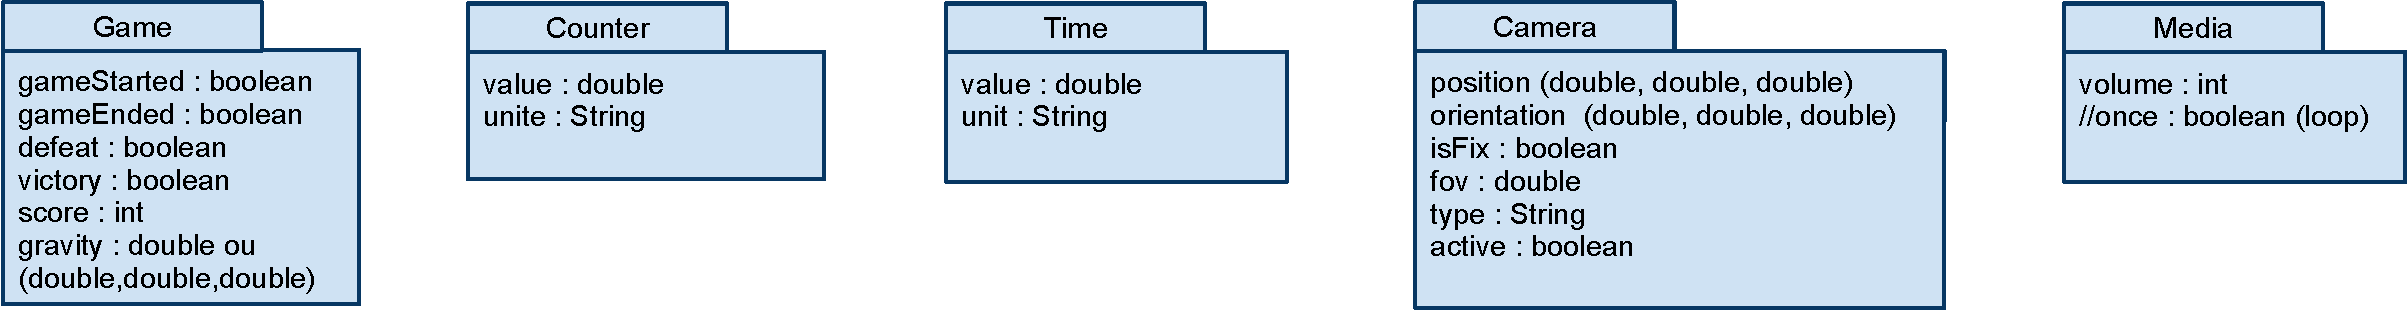
\includegraphics[width=\textwidth]{img/otherclass}
\end{figure}

La classe Game ne peut être instancier qu'une unique fois.

Les ressources temporelles peuvent avoir plusieurs unités telles que les secondes, les milisecondes ou les minutes.

Les caméras ont des types prédinis comme 'firstPreson' pour un suivi à la première personne, 'thirdPerson' pour un suivi à la troisième personne, ou 'free'
pour une caméra libre.

Un media a des mots-clefs dédiés comme play, mute on, mute off, pause ou stop.
Un attribut permet aussi de choisir entre un media répété en boucle ou lu une unique fois.

\subsection{La grammaire}

\begin{lstlisting}[language=Grammar]

/*------------------------------------------------------------------
* PARSER RULES
*------------------------------------------------------------------*/
 
game :
  (infosJeu '.')?
  (nouveauType '.')*
  (init '.')+
  (definition '.')*
  (commande '.')*
  (reglesJeu '.')*
  (iaBasique '.')*;
 

///////////////////////////// ( information of the game)  //////////////////////////////////

infosJeu :
  'game' 'has' ('gravity' | 'score' /*| ...*/ ) 'at' (NUMBER | NUMBER NUMBER NUMBER)
  ;

 
//////////////////////////// ( Inheritance )  /////////////////////////////
 
nouveauType :
  'type' ident 'is' (ident | typeObjet) ('and' ident | typeObjet)* // to declare a new type
  ;            
  
// ident | typeObjet : if it is an ident, verify that it is defined before by the user and is inherited Object.

 
//////////////////////////// ( Initialization )  /////////////////////////////

init :
  ident 'is' declarationObjet
  | accesClasse 'has' affectationObjet (',' affectationObjet)* // check the types and its attributes
  ;
 
declarationObjet :
  (ident | typeObjet3D) ('player' | interaction ('multiple')? )?         // interaction is neutral by default
  | 'list' ('of' (operation)? (ident) ('with' (operation)? (ident))* )?  //operation if it is multiple 
  | 'camera' (('first' | 'third') 'person' | 'free')
  | 'media' ('loop' | 'once')? 						 // sounds played in loop or once
  | 'in' ident 				                                 // ident of a list to add an element
// | ...)
;           
 
interaction :
  'ally' | 'enemy' | 'neutral'
  ;
 
affectationObjet :
  ident ('at' (operation (uniteTps)? | ident) )?         //aggregation
  | attribut 'at' (operation | STRING | BOOL)          //life at 5, name at "Gandalf Le Gris"
  | typeCoordonnees 'at' coordonnees            //size at 20 30 40
  | attributListeOuObjet 'at' ident             //inventory at listeArmesJoueur
  | attributTps 'at' operation uniteTps         //
  ;
 
// has ident at ... : to declare a new attribute
// Attributes of predefined class have default initialized
// it is not necessary to initialize not used attribute
  
typeObjet :
  'camera'
  | 'media'
  | 'counter'
  | 'time'
  | typeObjet3D
  ;
 
// all the predefined classes
typeObjet3D:
  'object'                      // -> position(x,y,z), orientation(x,y,z), taille(x,y,z)
  | 'character'                 // -> life, lifeMax, mana, manaMax , level, experience, attack, defense
  | 'vehicle'                   // -> acceleration, speedMax,
  | 'plane' | 'spaceCraft'
  | 'obstacle'                  // a fixed entity, used for collision
  | 'weapon'                    // -> nbMunitions, nbMaxMunitions, intervalleTirs, timeRecharge
  | 'sword'                     // -> damages, level
  | 'projectile'                // -> vitesse, damages, level(pourquoi pas)
  | 'zone'                      // an invisible and traversable entity
  | 'ground'                    // -> type of ground (water, snow ...)
  | 'bonus'                     // an object which disappears when something touches it-> valeur(entier), nomObjet(type),listeObjets 
  | 'checkPoint'
  | 'breakable'
  | 'construction'
  | 'room'
  | 'ball'
  | 'teleporter'
// | ...
  ;
 
// all the attributes of predefined classes
attribut : 
  'mass'                  // attributes of object :
  | 'isFix'
  | 'isTraversable'
  | 'fov'                    // attributes of "camera"
  | 'type'
  | 'active'
  | 'name'                   // attributes of "personnage" :
  | 'description'
  | 'life'
  | 'lifeMax'
  | 'lifeMin'   
  | 'nbOfLives'   
  | 'magic'
  | 'magicMax'
  | 'magicMin'
  | 'level'
  | 'attack'
  | 'defense'
  | 'jumpForce'
  | 'maxJumpsInTheAir'
  | 'money'
  | 'class'
  | 'race'
  | 'acceleration'    
  | 'speed'                // attributes of "vehicle" :
  | 'maxSpeed'
  | 'minSpeed'
  | 'boost'
  | 'maxBoost'
  | 'nbMunitions'           // attributes of"weapon" :
  | 'nbMunitionsMax'        
  | 'shootPower'
  | 'damages'               //attributes of "projectile"
  | 'value'                // attributes of "bonus" :
  | 'unit'
  | 'objectname'
  | 'attributName'               
  | 'volume'                 //attributes of "media"
  | 'number'              //attributes of "ball"
  | 'moveWithCamera'
// | ...
  ;
 
attributListeOuObjet :
  'inventory'
  | 'equipedObjects'
  | 'entrances'
  | 'exits'
  | 'damageZone'
  | 'collectors'
  | 'typesCollectors'
  | 'generators'
  | 'typeGenerators'
  | 'breakers'
  | 'typesBreakers'
  | 'teleportables'
  | 'typesTeleportables'
  ;
 
attributTps :
  'boostInterval'
  | 'shootInterval'        //attributes of "weapon" :
  | 'reloadTime'
// | ...
  ;
 

//////////////////////////// ( new definitions of actions ) ///////////////////
 
definition : 'definition' ident 'means' consequences;
 
consequences :
  consequ (',' consequ)*
  ;
  
consequ :
  siAlors
  | action
  | affectation
  | activCommande
  | appelDef
  | 'victory'
  | 'defeat'
// | ...
  ;
 
appelDef :
  ident           //ident of a definition of an action (means)
  ;
 
activCommande :
  ('activate' | 'disable') ('commands' | 'mouse' (souris (',' souris)*)? | 'key' clavier (',' clavier)* | 'keyboard' )
  ;
//disable commands              // all the commands
//disable key                   // all the key commands
//disable mouse up, down        // only move up or down with the mouse
 

//////////////////////////// ( Initialization of commands )  /////////////////////////////

commande :
  'command' (ident 'is' actionCommande (',' actionCommande)* | actionCommande)
  ;

actionCommande :
  ('mouse' souris | 'key' clavier) 'for' (ident | actionCommandePressee | actionCommandeMaintenue) // ident : what is defined with means
  ;
 
souris :
        'up' | 'down' | 'left' | 'right' | 'lClick' | 'cClick' | 'rClick' | 'scrollUp' | 'scrollDown'
        ;
 
clavier :
        CHAR | 'up' | 'down' | 'left' | 'right' | 'space' | 'echap' | 'enter'          //CHAR : Z,Q,S,D,...
        ;
 
actionCommandePressee :
  'jump'
  | 'pause'
  | 'stop'
// | ...
  ;
actionCommandeMaintenue :
  'move left'
  | 'move right'
  | 'move forward'
  | 'move backword'
  | 'accelerate'
  | 'brake'
  ;
 
 
//////////////////////////// ( Rules of game + victory condition / defeat )  /////////////////////////////

reglesJeu :
  'rule' (ident 'is')? declencheur 'then' consequences ','
  ;
conditions :
  conditionEt ('or' conditionEt)*
  ;
 
conditionEt :
  cond ('and' cond)*
  ;
  
cond         :
  etat
  | operation comparaison operation

etat :
  accesClasse 'is' ('not')? ('dead' | 'alive' | 'effaced' | 'generated' | 'touching' (('other')? accesGlobal | accesLocal))  // for an object
  | (ident | 'game') 'is' ('not')? ('finished' |'started' | 'paused' | 'muted' ('on' | 'off') | 'played' | 'stopped' )  // game,counter,media
  | 'true'                                                   
  | 'victory'
  | 'defeat'
  //  | ...
  ;
 
declencheur :
  accesClasse ('dies' | ('touches' | 'kills') (('other')? accesGlobal | accesLocal) | ('killed' | 'touched') ('by' (('other')? accesGlobal | accesLocal))? )
  | (ident | 'game') ('ends' |'starts')
  | variable 'becomes' varOuNb
  | ident 'becomes' ('player' | interaction)
// | ...         //ident if it is a counter
  ;
  
siAlors :
  'if' conditions 'then' consequences ('else' consequences)? 'end'
  ;
  
 
action :
  accesClasse actionObjet
  | (ident | 'game') ('ends' |'starts')
  | ('pause' | 'mute' ('on' | 'off') | 'play' | 'stop' ) ident
  | 'block' transformation 'of' accesClasse coordonnees
  | ('efface' | 'generate') (accesClasse | operation accesClasse ('in' accesLocal | 'on' accesLocal | 'at' coordonnees)?)
  | 'wait' operation uniteTps 'then' consequences 'endWait'
  | 'save'
// | ...
  ;
 
actionObjet :
  'dies'
  | actionCommandePressee
  | actionCommandeMaintenue ('during' operation uniteTps | 'until' conditions)
  | 'equip' (accesLocal | 'next' | 'previous')   
// | ...
  ;
 
affectation :
  (('assign' | 'add' | 'sub') operation) 'for' variable | 'invert' variable 'with' variable
  ;
/*
add : a += b, remove : a -= b, assign : a = b, invert : tmp=a; a=b; b=tmp;
*/
coordonnees :
  operation operation operation
  ;
 
comparaison :
  '=' | '<' | '>' | '<=' | '>='
  ; 
 
transformation :
  'translation'
  | 'rotation'
  | 'scale'
  ;
 
uniteTps :
  'mn'
  | 'sec'
  | 'ms'
  | 'frames'
  ;
 
operation :
  ('random' 'between' operationPlus 'and')? operationPlus
  ;
 
operationPlus :
  operationMul (operateurPlus operationMul)*
  ;
operationMul :
  operationPuiss (operateurMul operationPuiss)*
  ;
  
operationPuiss :
  operationparentheses ('^' operationparentheses)*
  ;
  
operationparentheses :
  '(' operation ')'
  | varOuNb
  ;
 
varOuNb :
  variable
  | NUMBER
  ;
 
variable :
  (('x' | 'y' | 'z') 'of' (typeCoordonnees | ident | attribut)) 'of' accesClasse
                      //x of size of num 10 in listeWeapon
// | ...
  ;
 
accesClasse : accesLocal | accesGlobal;
 
accesGlobal :
  typeObjet
  | interaction
  | 'not' (typeObjet | interaction | 'player')
  | 'all'
  ;
 
accesLocal :
  ident
  | 'num' operation 'in' ident
  | 'player'
  ;
 
 
typeCoordonnees :
  'positition' | 'rotation' | 'scale'
  ;
 
operateur :
  operateurMul
  | operateurPlus
  ;
  
operateurMul :
  '*'
  | '/'
  | '%'
  ;
  
operateurPlus :
  '+'
  | '-'
  ;
 
ident :
  STRING
  ;
 
//////////////////////////// ia //////////////////////////
 
iaBasique : 'ia' accesClasse 'is' actionObjet (',' actionObjet)*;
 

/*------------------------------------------------------------------
* LEXER RULES
*------------------------------------------------------------------*/
BOOL        : ('true' | 'false');
STRING        :  ('a'..'z' | 'A'..'Z') ('a'..'z' | 'A'..'Z' | '0'..'9')+ ;
CHAR   : 'a'..'z' | 'A'..'Z';
NUMBER : ('0'..'9')+ (',' ('0'..'9')+ )? ;
WS  :   ( ' '  
           | '\t'  
           | '\r'  
           | '\n'  
           | '\u000C'
           )+ {$channel=HIDDEN;}  
        ;
\end{lstlisting}
